\documentclass{article}

\usepackage{amsmath}
\usepackage{graphicx}
\usepackage{courier}

\begin{document}
	\title{E4301 Final Project: Spectral Solution to the Klein-Gordon Equation}
	\author{Stephen Carr and Brian Dawes}
	\date{\today}
	\maketitle
	
	\begin{abstract}
		filler text
	\end{abstract}
	
	\section*{1. Introduction}
	
	
	The Klein-Gordon Equation appears in many subfields of physics, most notably in particle physics, where it is the relativistic generalization of the Schr\"odinger Wave equation. We wish to study it in a slightly different context, namely as the generalization of Maxwell's Equations for massive photons. We wish to see how the solutions to the Klein-Gordon forumlation deviate from the classical E\&M results.
	
	We will use the following set of equations as our (uncoupled) PDE for the E and B fields in a vacuum (which can be derived from the coupled Massive Maxwell Equations, omitted here):
	\begin{equation}
	\boxed{
		\left(\frac{1}{c^2}\frac{\partial^2}{\partial t^2} - \nabla^2 + m^2\right)
		\begin{pmatrix}
		\vec{E} \\
		\vec{B}
		\end{pmatrix}
		=
		\begin{pmatrix}
		-4\pi\nabla\rho - \frac{4\pi}{c^2}\frac{\partial\vec{j}}{\partial t} \\
		\frac{4\pi}{c}(\nabla\times\vec{j})
		\end{pmatrix}
	}
	\end{equation}
	
	Here, $c$ represents the speed of light, which is the propagation velocity for an EM wave in a vacuum. The $m$ represents the photon's mass (which we will leave as a variable parameter). Our source functions depend on $\rho$, the charge density, and $\vec{j}$, the current density, both of which are functions of position and time. These sources will be fixed, and we will try various combinations in increasing complexity. The goal of this modeling is to investigate how the propagation of Electro-Magnetic waves depends on the mass term.
	\section*{2. Implementation}
	
	Like the standard wave-equation, the Klein-Gordon wave equation can be simplified from a second order PDE to a second order ODE by taking the Fourier Transform in space. In this form, $\vec{E} = \sum_{k}\vec{E_k}$, $\nabla^2 = -k^2$, and $\nabla = -i\vec{k}$:
	
	\begin{equation}
		\left(\frac{1}{c^2}\frac{\partial^2}{\partial t^2} + k^2 + m^2\right)\vec{E_k} = 4\pi i \vec{k} \rho_k - \frac{4\pi}{c^2}\frac{\partial\vec{j_k}}{\partial t} = \vec{F_k}(\vec{x},t)
	\end{equation}
	
	Thus, in Fourier space our problem completely diagonalizes into a set of independent equations in $k$.
	Using a standard stencil for the 2nd order derivative, with $n$ our time index and $h$ our time-step, and letting $\phi$ represent one of the three componenets of $\vec{E}$:
	
	\begin{equation}
		\frac{\partial^2 \phi_k}{\partial t^2} = \frac{-\phi_k^{n+1} + 2\phi_k^{n} - \phi_k^{n-1}}{h^2}
	\end{equation}
	
	Solving for $\phi_k$ we get our functional equation:
	
	\begin{equation}\boxed{
		\phi_k^{n+1} = 2\phi_k^n - \phi_k^{n-1} + c^2h^2(F_k - (k^2+m^2)\phi_k^n)}
	\end{equation}
	
	This form is implemented in a python script on a truncated spectral space of size $N^3$ (i.e. look only at wavenumbers $2\pi m/N$ for $m \in [0,N-1]$). Then a second python script for plotting the Electric Field components and total Energy distribution (Energy proportional to $\vec{E}^2$) was used for analyzing our solution in position-space.
	
	\section*{3. Stability and Convergence}
	
	Initially, we tried to input a Dirac delta-function as our source with an inital condition of zero everywhere. But then the source $F_k \approx \vec{k}$ which caused the first step of ou problem to act like $\phi_k^{1} = c^2h^2 F_k \approx c^2h^2k$ and then at the large k values of subsequent steps $\phi_k^{n+1} \approx -c^2h^2k^3\phi_k^n$.
	
	\begin{center}
		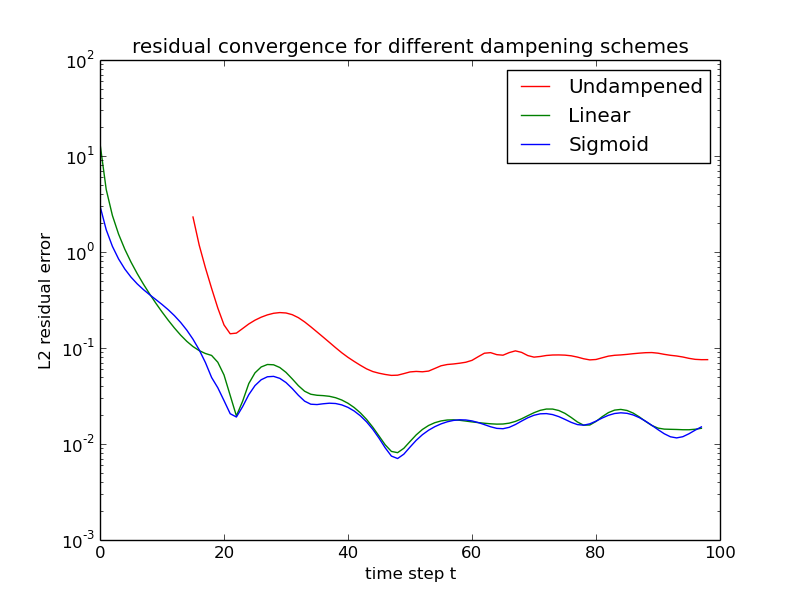
\includegraphics[width=5in]{conv_plot_100}
		
		Stability plot
		
	\end{center} 
	
	Stability: show the "steadystate" convergence plots, discuss the point source shock problem.
	
	Convergence: no analytic problem to compare to for the stable forms, so qualitatively compare the "tail" of the energy or electric field.
	
	\section*{4. Simulations}
	
	mass dependence
	
	interesting charge sources
	
	interesting current sources
	
	\section{5. Conclusion}
	Summary of successes in relation to original goal
	
	Improvements
	
	What we would like to also implement
	
\end{document}